% ------------------------------------------------------------------------------
% TYPO3 Version 9.1 - What's New - Chapter "Backend User Interface" (Serbian Version)
%
% @author	Michael Schams <schams.net>
% @license	Creative Commons BY-NC-SA 3.0
% @link		http://typo3.org/download/release-notes/whats-new/
% @language	English
% ------------------------------------------------------------------------------
% LTXE-CHAPTER-UID:		07b25346-95b1df21-a6ebe09a-49f53f41
% LTXE-CHAPTER-NAME:	Backend User Interface
% ------------------------------------------------------------------------------

\section{Administratorski interfejs}
\begin{frame}[fragile]
	\frametitle{Administratorski interfejs}

	\begin{center}\huge{Poglavlje 1:}\end{center}
	\begin{center}\huge{\color{typo3darkgrey}\textbf{Administratorski interfejs}}\end{center}

\end{frame}

% ------------------------------------------------------------------------------
% LTXE-SLIDE-START
% LTXE-SLIDE-UID:		be47f964-49ceaed9-ecc4001c-7719488a
% LTXE-SLIDE-ORIGIN:	e0ad33fe-9f5b1a93-218b12e9-6410e8f5 English
% LTXE-SLIDE-TITLE:		Added New Main Module Site Management
% LTXE-SLIDE-REFERENCE:	Feature-83637-AddedNewMainModuleSiteManagement.rst
% ------------------------------------------------------------------------------

\begin{frame}[fragile]
	\frametitle{Administratorski interfejs}
	\framesubtitle{Upravljenje sajtovima (Site Management)}

	Dodat je novi modul \textbf{Site Management} u TYPO3.
	Uloga ovog modula je da se u njemu nalaze konfiguracije sajtova, na primer jezik, domeni i rutiranje.
	\begin{columns}[T]
		\begin{column}{.4\textwidth}
			\begin{figure}\vspace*{-0.4cm}
				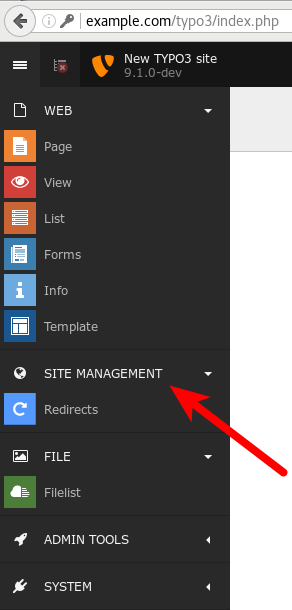
\includegraphics[width=0.45\linewidth]{BackendUserInterface/AddedNewMainModuleSiteManagement.png}
			\end{figure}
		\end{column}
		\begin{column}{.5\textwidth}
			Nova sistemska ekstenzija \texttt{EXT:redirects} je prva komponenta ovog modula (detalji su na sledecoj stranici).
		\end{column}
		\begin{column}{.1\textwidth}
		\end{column}
	\end{columns}

\end{frame}

% ------------------------------------------------------------------------------
% LTXE-SLIDE-START
% LTXE-SLIDE-UID:		c2f0ecdb-089250d1-26426892-367ac9c8
% LTXE-SLIDE-ORIGIN:	8bd6b85d-ed8c77e3-94a40b39-e15bb504 English
% LTXE-SLIDE-TITLE:		System Extension "Redirects" Has Been Added
% LTXE-SLIDE-REFERENCE:	Feature-83631-SystemExtensionRedirectsHasBeenAdded.rst
% ------------------------------------------------------------------------------

\begin{frame}[fragile]
	\frametitle{Administratorski interfejs}
	\framesubtitle{Redirekcije (Redirects)}

	Novi modul omogucava integratorima i editorima da konfigurisu redirekcije.
	Funkcija ima jednostavan brojac poseta (treba da se omoguci) 
	i moze da se unese neogranicen broj redirekcija u toku odredjenog perioda vremena.

	\begin{figure}
		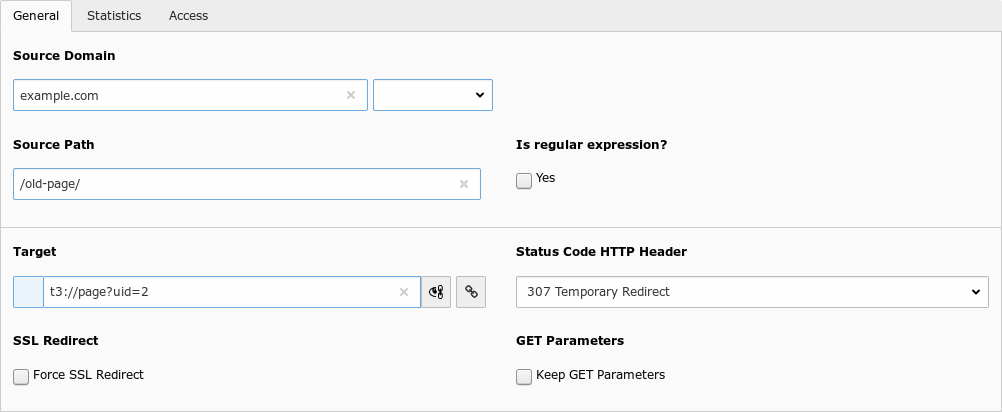
\includegraphics[width=0.8\linewidth]{BackendUserInterface/SystemExtensionRedirectsHasBeenAdded.png}
	\end{figure}

\end{frame}

% ------------------------------------------------------------------------------
% LTXE-SLIDE-START
% LTXE-SLIDE-UID:		dbf03c63-d9b44c52-e0371eb8-e3427ec3
% LTXE-SLIDE-ORIGIN:	e10a0f89-e91ecdb3-928841b6-1a84fc50 English
% LTXE-SLIDE-TITLE:		Show Fieldname Next To Title In Debug Mode
% LTXE-SLIDE-REFERENCE:	Feature-83461-ShowFieldnameNextToTitleInDebugMode.rst
% ------------------------------------------------------------------------------

\begin{frame}[fragile]
	\frametitle{Administratorski interfejs}
	\framesubtitle{Imena polja u Debug modu}

	\begin{itemize}

		\item TYPO3 integratori i programeri cesto se susrecu sa poljima za unos u administratorskom interfejsu,
			na primer kada se konfigurisu permisije ili tokom konfiguracije TsConfig.

		\item Umesto da se gleda u kod pretrazivaca, imena polja se prikazuju za svako polje generisano pomocu FormEngine-a.

		\item Ovo vazi samo za administratore pod uslovom da je ukljucen debug mod u TYPO3:

			\smaller
				\texttt{\$GLOBALS['TYPO3\_CONF\_VARS']['BE']['debug']}
			\normalsize

	\end{itemize}

	\begin{figure}
		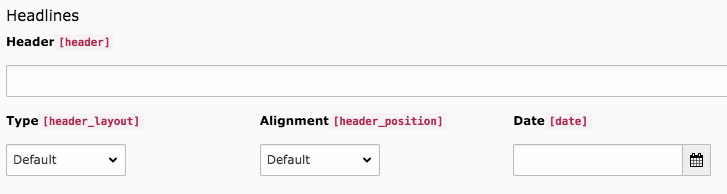
\includegraphics[width=0.60\linewidth]{BackendUserInterface/ShowFieldnameNextToTitleInDebugMode.png}
	\end{figure}

\end{frame}

% ------------------------------------------------------------------------------
